\section{Stockage des documents}

Le projet comportant de nombreux livrables à portée interne comme externe, il est donc nécessaire de mettre en place une gestion de la documentation, simplifiant ainsi la gestion des livrables. Un espace de stockage est tout d’abord nécessaire afin de sauvegarder et d’archiver les différents documents produits par l’équipe travaillant sur le projet. Pour cela, l’outil Google Drive sera utilisé, donnant ainsi accès à tous les membres de l’équipe aux documents du projet. Afin de faciliter davantage l’organisation des documents, un dossier par phase (initialisation, expression du besoin…) sera créé sur cet espace de stockage, en addition du dossier spécifique aux tâches de gestion de projet.
 
\begin{figure}[H]
    \centering
    \label{fig-arbo}
    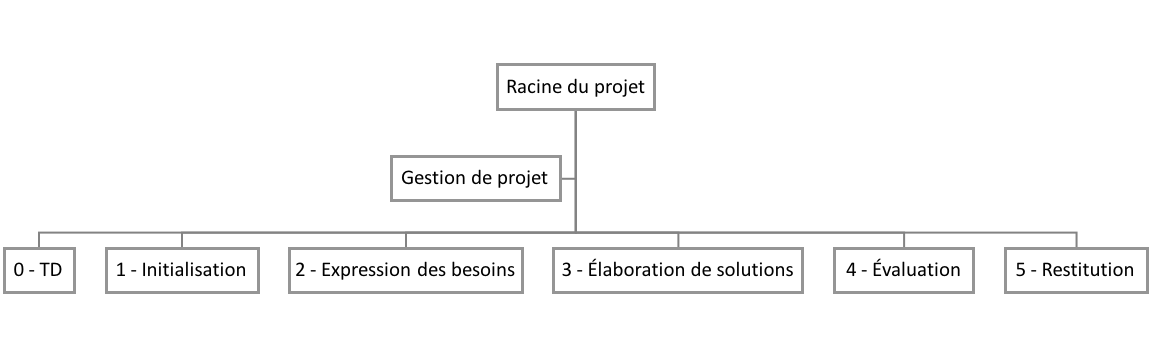
\includegraphics[scale=0.65]{figures/arbo.png}
    \caption{Hiérarchie des documents sur Google Drive }
\end{figure}

\section{Collaboration de la rédaction}

En combinaison avec l’espace de stockage Google Drive, l’outil Google Docs sera également utilisé pour créer et éditer les différents documents texte, tandis que l’outil Google Sheets sera utilisé pour les feuilles de calcul. Ces deux outils collaboratifs permettent de travailler à plusieurs sur les documents, tout en réalisant une gestion d’historique. Ainsi, des vérifications à intervalles réguliers seront effectuées sur les documents, ces derniers étant facilement accessibles.
 
\section{Mise en forme et stockage final}

Lorsqu’un document est en version finale (se référer au paragraphe « Cycle de vie des documents » pour plus d’information), celui-ci est pris en charge par la qualité, qui débute le processus de recette. Lors de cette étape, le responsable qualité transforme le document Google Docs (ou Google Sheets, le cas échéant) afin d’obtenir un document au format LaTeX, garantissant ainsi l’uniformité des livrables. Le document au format LaTeX est ensuite transformé en fichier au format PDF, représentant ainsi la version de recette. Ces documents au format LaTeX et PDF sont ensuite archivés sur un dépôt Git, permettant ainsi de prévoir une gestion des versions de recette tout en proposant une sauvegarde distante.

Enfin, la livraison des documents finaux, au format PDF, sera effectuée via la plateforme Moodle, qui comporte les différents dépôts de données associés aux livrables attendus par le client. \\

Ainsi, les changements de format des différents documents produits au sein du projet peuvent être résumés à travers le schéma ci-dessous, de la création collaborative à l’archivage et la livraison de la version transformée au format PDF.

\begin{figure}[H]
    \centering
    \label{fig-conversion}
    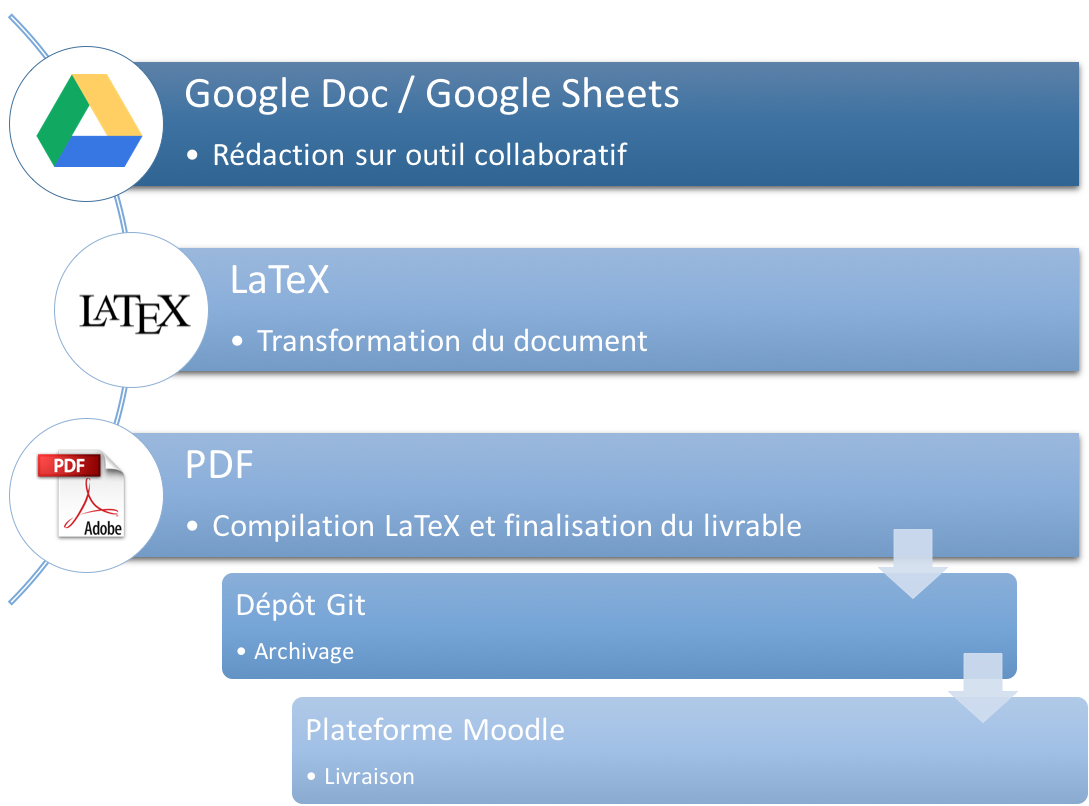
\includegraphics[scale=0.5]{figures/conversion.png}
    \caption{Formats et dépôt d’un livrable durant son cycle de vie}
\end{figure}